\usetikzlibrary{shapes.geometric}


\begin{figure}
\centering
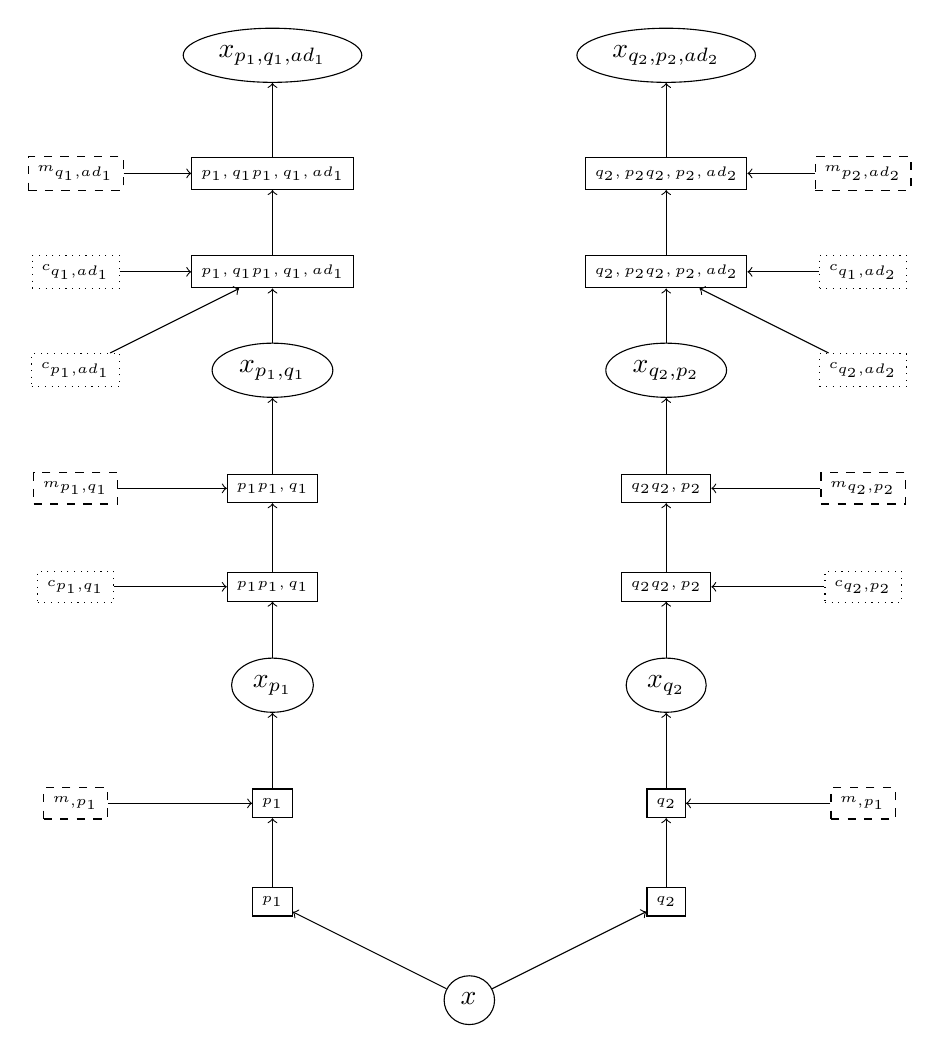
\begin{tikzpicture}
  \tikzset{
    _x/.style={ellipse,draw},
    r/.style={rectangle,draw,font=\tiny},
    m/.style={rectangle,draw,dashed,font=\tiny},
    c/.style={rectangle,draw,dotted,font=\tiny},
  }

  \node[_x] (x-null)    at (0,0)  {$x_{\varnothing}$};
  \node[_x] (x-p1)      at (-2.5,4) {$x_{ \set{p_1} }$};
  \node[_x] (x-p1q1)    at (-2.5,8) {$x_{ \set{p_1,q_1} }$};
  \node[_x] (x-p1q1ad1) at (-2.5,12) {$x_{ \set{p_1,q_1,ad_1} }$};
  \node[_x] (x-q2)      at (2.5,4)  {$x_{ \set{q_2} }$};
  \node[_x] (x-q2p2)    at (2.5,8)  {$x_{ \set{q_2,p_2} }$};
  \node[_x] (x-q2p2ad2) at (2.5,12)  {$x_{ \set{q_2,p_2,ad_2} }$};

  \node[r] (rc-null-p1)      at (-2.5,1.25) {$\rc{\varnothing}{ \set{p_1} }$};
  \node[r] (rm-null-p1)      at (-2.5,2.5) {$\rM{\varnothing}{ \set{p_1} }$};
  \node[r] (rc-p1-p1q1)      at (-2.5,5.25) {$\rc{ \set{p_1} }{ \set{p_1,q_1} }$};
  \node[r] (rm-p1-p1q1)      at (-2.5,6.5) {$\rM{ \set{p_1} }{ \set{p_1,q_1} }$};
  \node[r] (rc-p1q1-p1q1ad1) at (-2.5,9.25) {$\rc{ \set{p_1,q_1} }{ \set{p_1,q_1,ad_1} }$};
  \node[r] (rm-p1q1-p1q1ad1) at (-2.5,10.5) {$\rM{ \set{p_1,q_1} }{ \set{p_1,q_1,ad_1} }$};

  \node[r] (rc-null-q2)      at (2.5,1.25) {$\rc{\varnothing}{ \set{q_2} }$};
  \node[r] (rm-null-q2)      at (2.5,2.5) {$\rM{\varnothing}{ \set{q_2} }$};
  \node[r] (rc-q2-q2p2)      at (2.5,5.25) {$\rc{ \set{q_2} }{ \set{q_2,p_2} }$};
  \node[r] (rm-q2-q2p2)      at (2.5,6.5) {$\rM{ \set{q_2} }{ \set{q_2,p_2} }$};
  \node[r] (rc-q2p2-q2p2ad2) at (2.5,9.25) {$\rc{ \set{q_2,p_2} }{ \set{q_2,p_2,ad_2} }$};
  \node[r] (rm-q2p2-q2p2ad2) at (2.5,10.5) {$\rM{ \set{q_2,p_2} }{ \set{q_2,p_2,ad_2} }$};

  \node[m] (m-null-p1)       at (-5,2.5)  {$m_{\varnothing, p_1 }$};
  \node[m] (m-p1-q1)         at (-5,6.5)  {$m_{\set{p_1}, q_1 }$};
  \node[m] (m-q1-ad1)        at (-5,10.5) {$m_{\set{q_1}, ad_1 }$};

  \node[m] (m-null-q2)       at (5,2.5)  {$m_{\varnothing, p_1 }$};
  \node[m] (m-q2-p2)         at (5,6.5)  {$m_{\set{q_2}, p_2 }$};
  \node[m] (m-p2-ad2)        at (5,10.5) {$m_{\set{p_2}, ad_2 }$};

  \node[c] (c-p1-q1)         at (-5,5.25) {$c_{ p_1,q_1 }$};
  \node[c] (c-p1-ad1)        at (-5,8)    {$c_{ p_1,ad_1 }$};
  \node[c] (c-q1-ad1)        at (-5,9.25) {$c_{ q_1,ad_1 }$};

  \node[c] (c-q2-p2)         at (5,5.25) {$c_{ q_2,p_2 }$};
  \node[c] (c-q2-ad2)        at (5,8)    {$c_{ q_2,ad_2 }$};
  \node[c] (c-p2-ad2)        at (5,9.25) {$c_{ q_1,ad_2 }$};

  \draw[->] (x-null)          -- (rc-null-p1);
  \draw[->] (rc-null-p1)      -- (rm-null-p1);
  \draw[->] (rm-null-p1)      -- (x-p1);
  \draw[->] (x-p1)            -- (rc-p1-p1q1);
  \draw[->] (rc-p1-p1q1)      -- (rm-p1-p1q1);
  \draw[->] (rm-p1-p1q1)      -- (x-p1q1);
  \draw[->] (x-p1q1)          -- (rc-p1q1-p1q1ad1);
  \draw[->] (rc-p1q1-p1q1ad1) -- (rm-p1q1-p1q1ad1);
  \draw[->] (rm-p1q1-p1q1ad1) -- (x-p1q1ad1);
  
  \draw[->] (x-null)          -- (rc-null-q2);
  \draw[->] (rc-null-q2)      -- (rm-null-q2);
  \draw[->] (rm-null-q2)      -- (x-q2);
  \draw[->] (x-q2)            -- (rc-q2-q2p2);
  \draw[->] (rc-q2-q2p2)      -- (rm-q2-q2p2);
  \draw[->] (rm-q2-q2p2)      -- (x-q2p2);
  \draw[->] (x-q2p2)          -- (rc-q2p2-q2p2ad2);
  \draw[->] (rc-q2p2-q2p2ad2) -- (rm-q2p2-q2p2ad2);
  \draw[->] (rm-q2p2-q2p2ad2) -- (x-q2p2ad2);

  \draw[->] (m-null-p1)       -- (rm-null-p1);
  \draw[->] (m-p1-q1)         -- (rm-p1-p1q1);
  \draw[->] (m-q1-ad1)        -- (rm-p1q1-p1q1ad1);

  \draw[->] (m-null-q2)       -- (rm-null-q2);
  \draw[->] (m-q2-p2)         -- (rm-q2-q2p2);
  \draw[->] (m-p2-ad2)        -- (rm-q2p2-q2p2ad2);

  \draw[->] (c-p1-q1)         -- (rc-p1-p1q1);
  \draw[->] (c-p1-ad1)        -- (rc-p1q1-p1q1ad1);
  \draw[->] (c-q1-ad1)        -- (rc-p1q1-p1q1ad1);

  \draw[->] (c-q2-p2)         -- (rc-q2-q2p2);
  \draw[->] (c-q2-ad2)        -- (rc-q2p2-q2p2ad2);
  \draw[->] (c-p2-ad2)        -- (rc-q2p2-q2p2ad2);
\end{tikzpicture}
\caption{Causal graph for the blacklist network}
\label{fig:blacklist:causal-graph}
\end{figure}
